\documentclass[12pt]{report}

%Vous souciez pas de tout les packages, j'ai oublié ce que fait la moitié d'entre eux

\usepackage[utf8]{inputenc}
\usepackage[T1]{fontenc}
\usepackage[francais]{babel}
%\usepackage{layout}
\usepackage[left=3cm,right=3cm,top=3cm,bottom=3cm]{geometry}
%\usepackage{setspace}
\usepackage{soul}
\usepackage[normalem]{ulem}
%\usepackage{eurosym}
%\usepackage{bookman}
%\usepackage{charter}
%\usepackage{newcent}
%\usepackage{lmodern}
%\usepackage{mathpazo}
%\usepackage{mathptmx}
%\usepackage{url}
%\usepackage{verbatim}
%\usepackage{moreverb}
%\usepackage{listings}
%\usepackage{fancyhdr}
%\usepackage{wrapfig}
\usepackage{color}
%\usepackage{colortbl}
\usepackage{amsmath}
\usepackage{amssymb}
\usepackage{mathrsfs}
%\usepackage{asmthm}
%\usepackage{makeidx}
\usepackage{graphicx}
\usepackage{tabularx}
\usepackage{tgtermes}
\usepackage{titlesec}
\usepackage[final]{pdfpages} 
\usepackage{epsfig}
\usepackage{comment}
\usepackage{float}
\usepackage{amsmath}
\renewcommand{\emph}{\textit}
\renewcommand{\thesection}{\arabic{section}}
\renewcommand{\thesubsection}{\arabic{section}.\arabic{subsection}}
\titleformat*{\subsection}{\bfseries}
\parskip=5pt

%Information pour la page de garde

\title{TP 1 - Introduction au codage d'image : EQM, PSNR, entropie, histogramme}
\author{Jean-Baptiste \bsc{Morice}, Guillaume \bsc{Versal}}
\date{\today}


\begin{document}



%Commande qui crée la page de garde
\maketitle

\tableofcontents

\newpage
\section*{Introduction}

Ce TP a pour objectif :
\begin{itemize}
\item la prise en main de la libraire OpenCV
\item la prise en main et la manipulation des outils permettant d'évaluer l'efficacité de codage. On travaillera sur la norme de compression JPEG principalement.\\
\end{itemize}
Pour ce TP, nous disposions d'une image de base représentant un smiley jaune au milieu. Il nous est fourni aussi trois exemplaires de cette images ayant été compressé au format JPEG mais chacune avec des niveaux de compression différents : 
\begin{itemize}
\item Une image à 80 de bonne qualité
\item Une image à 10  de qualité moyenne
\item Une image à 2 de mauvaise qualité\\
\end{itemize}
Dans la suite de ce TP, on étudiera l'impact de ces différents niveaux de compression sur l'image au travers différentes métriques tel que le PSNR ou le kurtosis.


\newpage
\section{Notre travail}

\subsection{Question 3.1}

Dans un premier temps nous devions mettre en place un programme lisant deux images et les convertissant du format RGB classique au format YCrCb et affichant les différents canaux. Le format YCrCb est un format utilisé notamment pour la télévision. Le canal Y correspond à l'information de luminance de l'image ( l'image en noir et blanc) et les canaux Cr et Cb porte les informations sur la couleur. 

Lorsque l'on applique ce programme à l'image originale et l'image Deg2 on obtient les résultats suivant :

%Image originale
\begin{figure}[H]
\begin{center}
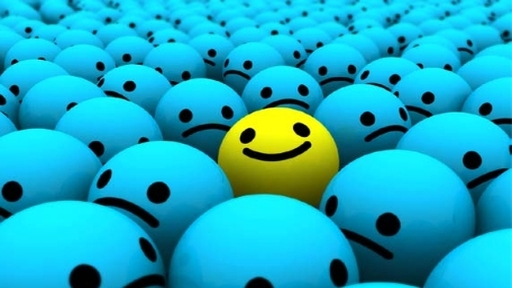
\includegraphics[scale=0.5]{../smiley.jpg} 
\caption{Image originale}
\end{center}
\end{figure}

\begin{figure}[H]
\begin{center}
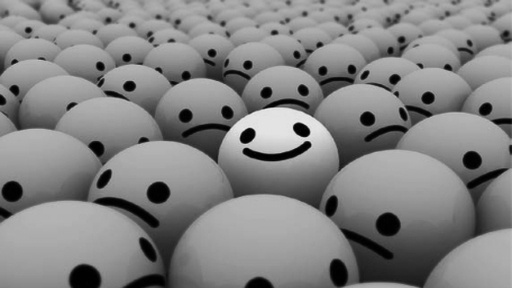
\includegraphics[scale=0.25]{../ImageRes/Image0_channel_0.jpg} 
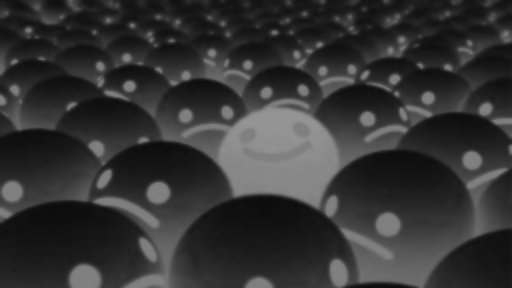
\includegraphics[scale=0.25]{../ImageRes/Image0_channel_1.jpg} 
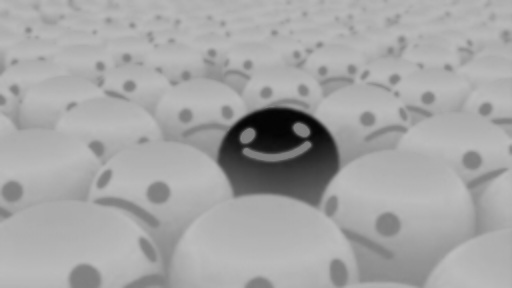
\includegraphics[scale=0.25]{../ImageRes/Image0_channel_2.jpg} 
\caption{Image originale selon les canaux Y, Cr et Cb}
\end{center}
\end{figure}

%Image avec Q2
\begin{figure}[H]
\begin{center}

\includegraphics[scale=0.5]{../smileyDegQ2.jpg} 
\caption{Image JPEG Q2}
\end{center}
\end{figure}

\begin{figure}[H]
\begin{center}
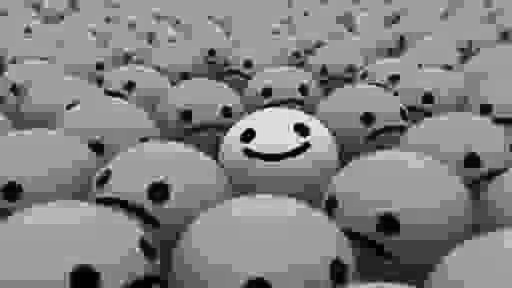
\includegraphics[scale=0.25]{../ImageRes/Image3_channel_0.jpg} 
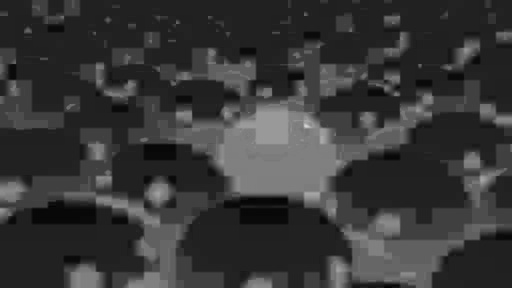
\includegraphics[scale=0.25]{../ImageRes/Image3_channel_1.jpg} 
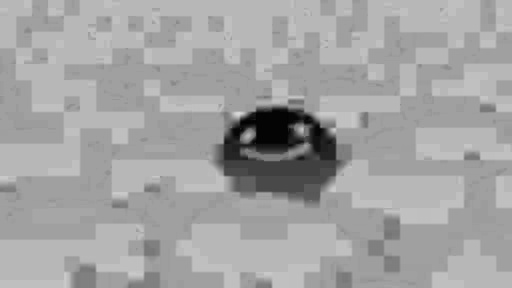
\includegraphics[scale=0.25]{../ImageRes/Image3_channel_2.jpg} 
\caption{Image JPEG Q2 selon les canaux Y, Cr et Cb}
\end{center}
\end{figure}

\subsection{Question 3.2 à 3.6}

Pour ces questions, nous devions mettre en place la métrique du PSNR et un élément plus visuel, la carte d'erreur, permettant de voir la différence entre deux images.

Le PSNR est un métrique faisant parti de la famille des "Full-Reference metrics" qui sont des métriques performantes mais nécessitant l'image originale et dégradée. Le PSNR calcul simplement la différence mathématique entre les pixels de chaque image (sans prendre en compte l'aspect visuel) et plus ce dernier est important plus les deux images comparées sont semblables.

La carte d'erreur s'inscrit dans le même cadre que le PSNR et elle correspond simplement à la différence entre deux images.

Ainsi, pour les différentes images DegQ80, DegQ10 et DegQ2 nous obtenons les résultats suivant :\\

\newpage
\textbf{Image compressée JPEG Q80}

\begin{figure}[H]
\begin{center}
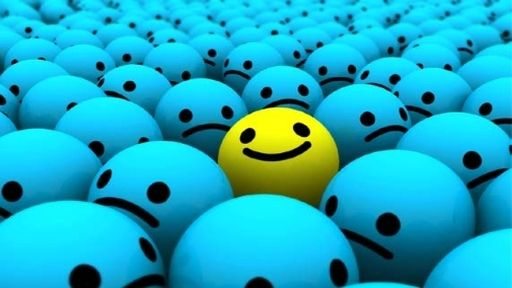
\includegraphics[scale=0.5]{../smileyDegQ80.jpg} 
\caption{Image compressée JPEG Q80 }
\end{center}
\end{figure}

\begin{figure}[H]
\begin{center}
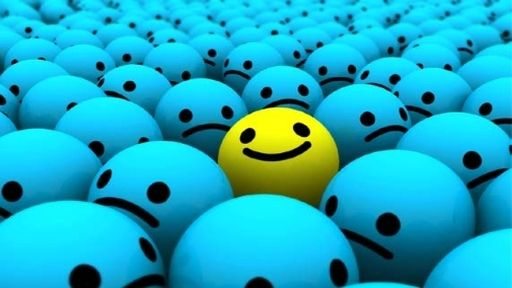
\includegraphics[scale=0.5]{../smileyDegQ80.jpg} 
\caption{Carte d'erreur de l'image compressée JPEG Q80 }
\end{center}
\end{figure}

Pour l'image compressée JPEG Q80 à un EQM de 4.71877 et un PSNR de 41.3925.\\

\textbf{Image compressée JPEG Q10}

\begin{figure}[H]
\begin{center}
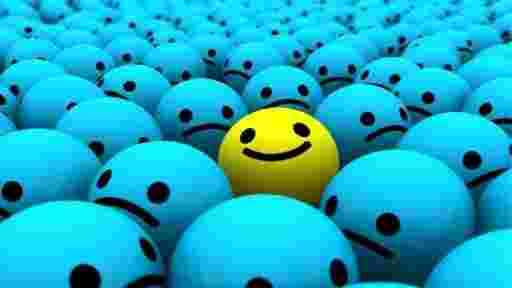
\includegraphics[scale=0.5]{../smileyDegQ10.jpg} 
\caption{Image compressée JPEG Q10 }
\end{center}
\end{figure}

\begin{figure}[H]
\begin{center}
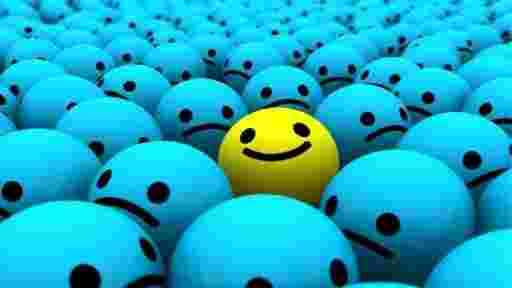
\includegraphics[scale=0.5]{../smileyDegQ10.jpg} 
\caption{Carte d'erreur de l'image compressée JPEG Q10 }
\end{center}
\end{figure}

Pour l'image compressée JPEG Q80 à un EQM de 52.1242 et un PSNR de 30.9604.\\

\textbf{Image compressée JPEG Q2}

\begin{figure}[H]
\begin{center}

\includegraphics[scale=0.5]{../smileyDegQ2.jpg} 
\caption{Image compressée JPEG Q2 }
\end{center}
\end{figure}

\begin{figure}[H]
\begin{center}

\includegraphics[scale=0.5]{../smileyDegQ2.jpg} 
\caption{Carte d'erreur de l'image compressée JPEG Q2 }
\end{center}
\end{figure}

Pour l'image compressée JPEG Q80 à un EQM de 246.224 et un PSNR de 24.2175.\\

Ainsi, si l'on trace la courbe de la taille du fichier en Bits en fonction du PSNR nous obtenons le résultat ci-dessous :

\begin{figure}[H]
\begin{center}
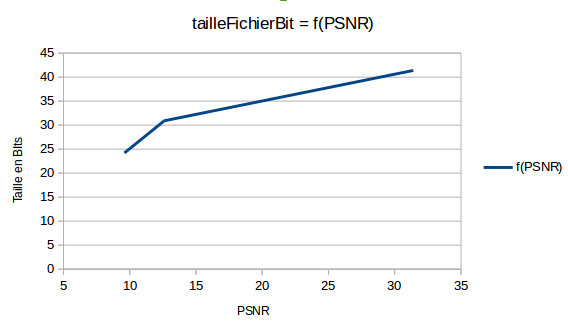
\includegraphics[scale=0.8]{../ImageRes/f(PSNR).png} 
\caption{Courbe taille en Bits en fonction du PSNR }
\end{center}
\end{figure}

Ce que l'on peut observer c'est que plus le PSNR augmente, plus le poids des images est conséquent. Ce qui est cohérent car plus le PSNR est faible, plus l'image originale est altérée pour prendre moins de place et donc plus l'EQM augmente.

On peut observer sur les images l'apparition d'un effet de bloc quand la compression devient très forte, c'est notamment très notable sur l'image DegQ2 ci-dessous.

\subsection{Question 3.5 et 3.6}

Dans la suite du TP, nous devions calculer l'entropie des images dégradée grâce au canal Y. L'entropie est une sorte d'indicateur de la complexité d'une image. Ainsi, une image uniforme dispose d'une entropie nulle tandis qu'une image riche aura une entropie élevée.

Après calcul, nous sommes à même de tracer la courbe entropie = f(niveau de compression) et nous obtenons le résultat suivant :

\begin{figure}[H]
\begin{center}
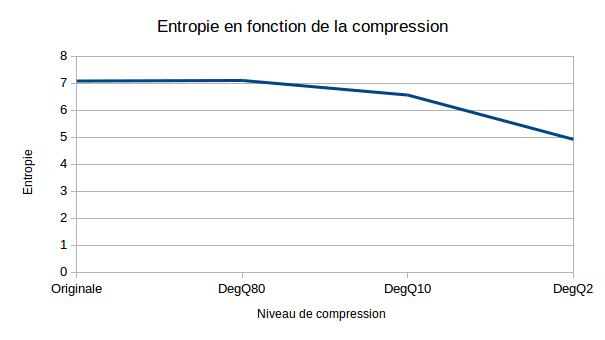
\includegraphics[scale=0.8]{../ImageRes/entropie.jpg} 
\caption{Entropie des images}
\end{center}
\end{figure}

On peut observer plusieurs chose sur ce graphique. Tout d'abord, entre l'image originale et le premier niveau de compression DegQ80 il n'y a pas de diminution de l'entropie, ce qui pourrait être étonnant. Cela est du au fait que comme le niveau de compression est très faible, la compression crée une sorte de bruit sur l'image et donc la rend plus aléatoire ce qui augmente l'entropie. 

C'est seulement à partir de DegQ10 que l'entropie des images commence à baisser doucement puis plus fortement avec DegQ2, le tout s'accompagnant de l'apparition d'effet de bloc.

\newpage
\subsection{Question 3.7 à 3.9}

Dans la dernier étape de notre TP est l'étude de l'histogramme des différentes images et voir quel impact à la compression sur ces derniers. Ainsi nous obtenons les histogrammes suivant :

\begin{figure}[H]
\begin{center}
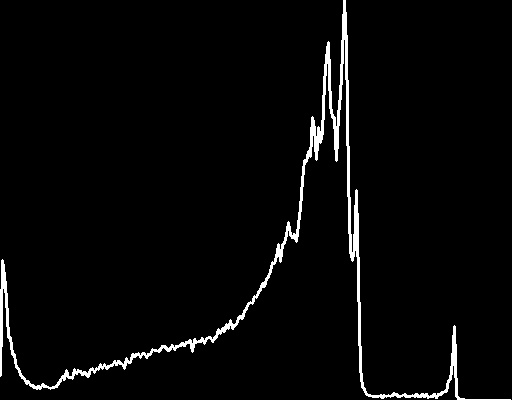
\includegraphics[scale=0.5]{../ImageRes/hist_0.jpg} 
\caption{Histogramme image originale}
\end{center}
\end{figure}

\begin{figure}[H]
\begin{center}
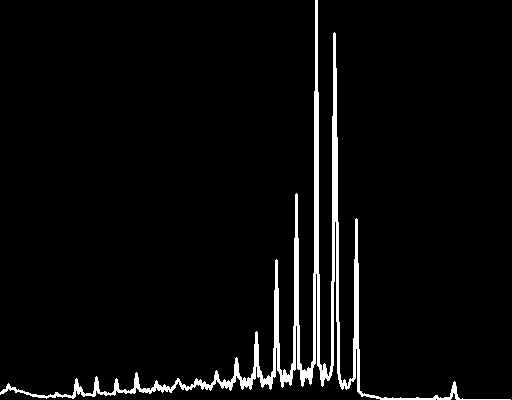
\includegraphics[scale=0.5]{../ImageRes/hist_1.jpg} 
\caption{Histogramme image dégradée Q80 }
\end{center}
\end{figure}

\begin{figure}[H]
\begin{center}
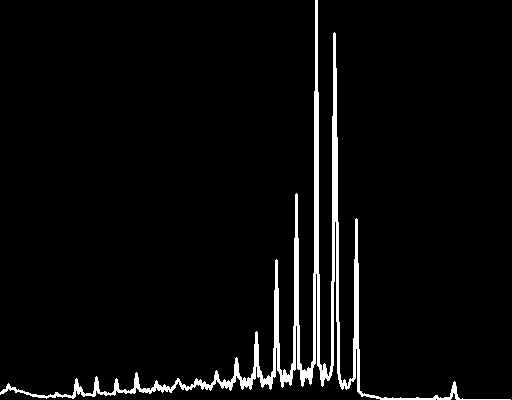
\includegraphics[scale=0.5]{../ImageRes/hist_2.jpg} 
\caption{Histogramme image dégradée Q10 }
\end{center}
\end{figure}

\begin{figure}[H]
\begin{center}
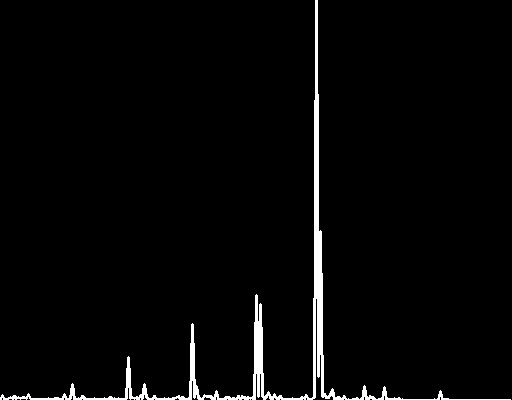
\includegraphics[scale=0.5]{../ImageRes/hist_3.jpg} 
\caption{Histogramme image dégradée Q2 }
\end{center}
\end{figure}

Nous pouvons observer sur ces différents histogrammes que plus la compression est forte, plus l'histogramme se retrouve "discrétisé autour de certaines valeurs. Cette effet est notamment très visible sur les images Q10 et Q2.

Pour finir, on décide de regarder et comparer les différents histogrammes des cartes d'erreur notamment via certaine métrique tel que le kurtosis.

\begin{figure}[H]
\begin{center}
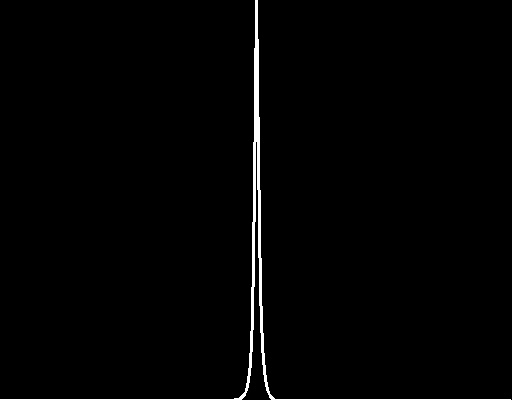
\includegraphics[scale=0.5]{../ImageRes/hist_disto_1.jpg} 
\caption{Histogramme carte d'erreur Q80 }
\end{center}
\end{figure}

\begin{center}
MeanHisto : 127.805\\
StandartDeviationHisto : 2.16352\\
KurtosisHisto : 8.20274
\end{center}

\begin{figure}[H]
\begin{center}
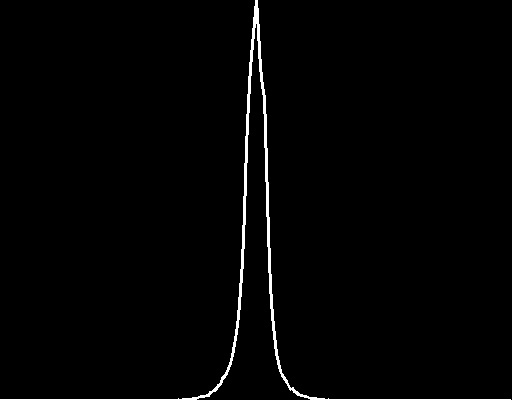
\includegraphics[scale=0.5]{../ImageRes/hist_disto_2.jpg} 
\caption{Histogramme carte d'erreur Q10 }
\end{center}
\end{figure}

\begin{center}
MeanHisto : 127.378\\
StandartDeviationHisto : 7.1929\\
KurtosisHisto : 7.63942
\end{center}

\begin{figure}[H]
\begin{center}
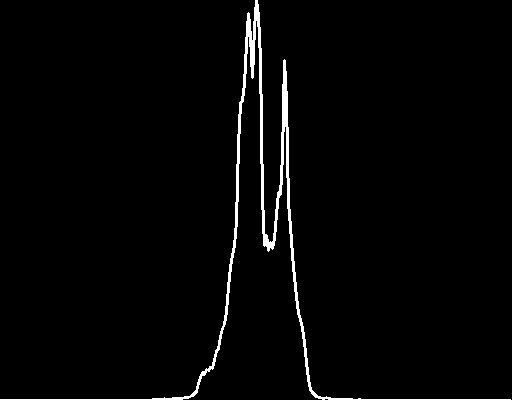
\includegraphics[scale=0.5]{../ImageRes/hist_disto_3.jpg} 
\caption{Histogramme carte d'erreur Q2 }
\end{center}
\end{figure}

\begin{center}
MeanHisto : 128.087\\
StandartDeviationHisto : 15.6906\\
KurtosisHisto : 7.2724
\end{center}

Ce que l'on peut observer c'est que la carte d'erreur de l'image DegQ80 dispose d'un histogramme semblable à un pic situé à 127,8, cela est du au fait que la différence avec l'image originale étant faible, les valeurs de la carte d'erreur tourne autour de 127,5. De plus, plus le niveau de compression augmente, plus l'histogramme de la carte d'erreur à tendance à s'étaler. Cette effet est notamment observable au travers de l'écart type que ne cesse d'augmenter plus on augmente la compression et du kurtosis qui diminue.

\newpage
Concernant l'entropie des cartes d'erreur, nous obtenons les résultats ci-dessous. Comme il est observable sur la courbe, plus la compression augmente, plus l'entropie de la carte d'erreur augmente. Cet effet est dû au fait que la différence avec l'image originale augmente et ainsi, le nombre de valeur que la carte d'erreur prend aussi.

\begin{figure}[H]
\begin{center}
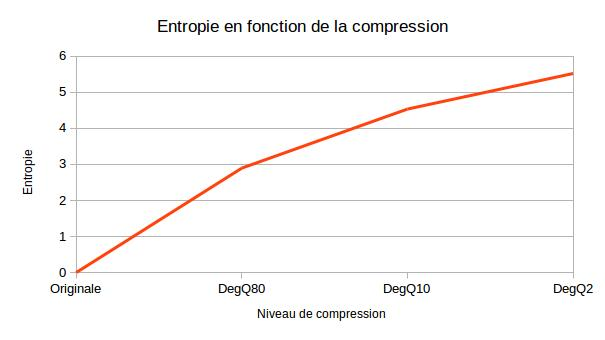
\includegraphics[scale=0.8]{../ImageRes/entropie_erreur.jpg} 
\caption{Entropie des images}
\end{center}
\end{figure}

\section{Conclusion}

Ce TP nous a permis de prendre en main la librairie OpenCV et de manipuler des outils d'évaluation d’efficacité de codage pour JPEG. Nous avons pu voir que plus la compression faite par JPEG dégrade la qualité de l'image soit en rajoutant du bruit, soit par la création d'effet de bloc. Cela était notamment observable sur les histogrammes et les images. Nous avons aussi pu observer que plus l'image est dégradé plus le PSNR de l'image augmente. L'utilisation du PSNR dans ce TP était  pertinent car l'image disposée de large zone uniforme mais cette métrique aurait pu ne pas convenir pour une image plus complexe, cette dernière étant purement mathématique.

Finalement, nous pouvons dire que la compression JPEG effectue bien son travail et réduit considérablement la taille de l'image mais cela se fait au détriment de la qualité. 

\begin{comment}

%Commande pour le sommaire

\renewcommand{\contentsname}{\large Sommaire} % Change le nom en sommaire
\setcounter{tocdepth}{2} % Défini la profondeur d'une table des matières
\tableofcontents
\newpage

\end{comment}

\newpage


%Commande pour le sommaire des figures

\renewcommand*\listfigurename{\large Liste des figures}
\listoffigures
\newpage


\end{document}